\begin{frame}{Fitting Procedure}
    Recall the general form of the PDE:
    \begin{equation}
        \frac{\partial u}{\partial t} + \mathcal{N}(u, \lambda) = 0
    \end{equation}

    and 

    \begin{equation}
        f := \frac{\partial u}{\partial t} + \mathcal{N}(u, \lambda)
    \end{equation}

We want to approximate $u(x, t)$ with a neural network $\hat{u}(x, t)$.

For this fitting we required two different sets of data:

\begin{itemize}
    \item Boundary conditions $\mathcal{X}_u$: Points where the solution of the PDE is known.
    \item Corresponding labels $\mathcal{Y}_u$ of the boundary conditions.
    \item Collocation points $\mathcal{X}_f$: Points where the PDE approximation should be valid.
\end{itemize}
\end{frame}

\begin{frame}{Fitting Procedure}
\framesubtitle{Data Sets}

\begin{figure}[H]
    \centering
    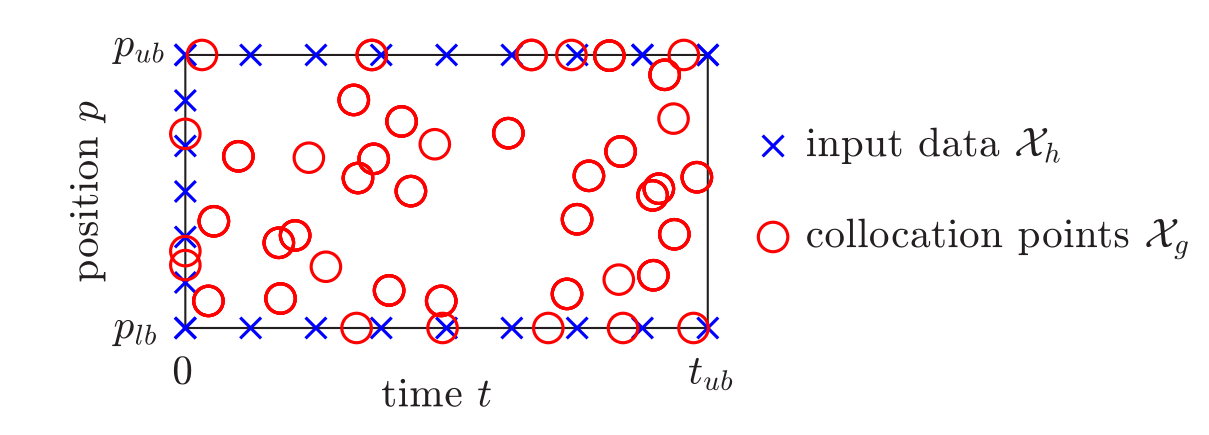
\includegraphics[width=0.8\textwidth]{img/space_time_grid.png}
    \caption{Space-Time grid points of the input data $\mathcal{X}_h$ and $\mathcal{X}_g$}
    \label{fig:space_time_grid}
\end{figure}   

\begin{align}
    \mathcal{X}_u &= \left\{
        \left(x_{u,1}, t_{u,1}\right),
        \cdots,
        \left(x_{u,i}, t_{u,i}\right),
        \cdots,
        \left(x_{u,n_u}, t_{u,n_u}\right)
    \right\}\\
    \mathcal{Y}_u &= \left\{
        u\left(x_{u,1}, t_{u,1}\right),
        \cdots,
        u\left(x_{u,i}, t_{u,i}\right),
        \cdots,
        u\left(x_{u,n_u}, t_{u,n_u}\right)
    \right\}
\end{align}

\begin{equation}
    \mathcal{X}_f = \left\{
        \left(x_{f,1}, t_{f,1}\right),
        \cdots,
        \left(x_{f,i}, t_{f,i}\right),
        \cdots,
        \left(x_{f,n_g}, t_{f,n_f}\right)
    \right\}
\end{equation}
\end{frame}

\begin{frame}{Fitting Procedure}
\framesubtitle{Loss Function}

We divide the loss function in two parts:

\begin{itemize}
    \item Loss function for the boundary conditions:
    \begin{equation}
        \mathcal{L}_u (\mathcal{X}_u, \mathcal{Y}_u, \hat{u}) = \frac{1}{n_u} \sum_{i=1}^{n_u} \left| u(x_{u,i}, t_{u,i}) - \hat{u}(x_{u,i}, t_{u,i})  \right|^2
    \end{equation}
    \item Loss function for the PDE:
    \begin{equation}
        \mathcal{L}_f (\mathcal{X}_f, \hat{u}, \hat{\lambda})= \frac{1}{n_f} \sum_{i=1}^{n_f} \left| \frac{\partial }{\partial t}\hat{u}(x_{f,i}, t_{f, i}) + \mathcal{N}(\hat{u}(x_{f,i}, t_{f, i}), \hat{\lambda}) \right|^2
    \end{equation}
\end{itemize}
\end{frame}

\begin{frame}{Fitting Procedure}
\framesubtitle{Total Loss Function}

The total loss function is given by:

\begin{equation}
    \mathcal{L}(\mathcal{X}_u, \mathcal{Y}_u,\mathcal{X}_f, \hat{u}, \hat{\lambda}) = \mathcal{L}_u (\mathcal{X}_u, \mathcal{Y}_u, \hat{u}) + \mathcal{L}_f (\mathcal{X}_f, \hat{u}, \hat{\lambda})
\end{equation}

And we aim to minimize it with respect to the parameters of the neural network $\hat{u}$ and the parameters of the PDE $\hat{\lambda}$.

\end{frame}